\section{Zadanie 6}
\subsection{Opis problemu}
Celem tego zadania było znalezienie miejsc zerowych funkcji $ f_1(x) = e^{1 - x} - 1 $ oraz $ f_2(x) = xe^{-x} $ za pomocą wcześniej zaimplementowanych metod przy dokładności $ \delta = 10^{-5}$, $\epsilon = 10^{-5}$. Dobrać odpowiednio przedział i przybliżenie początkowe.
\subsection{Rozwiązanie}

Na samym początku, dla ułatwienia zadania, za pomocą biblioteki $ \texttt{matplotlib} $ wygenerowałem wykresy funkcji $ f_1(x)$ oraz $f_2(x)$.

\begin{figure}[!htbp]
  \centering  
  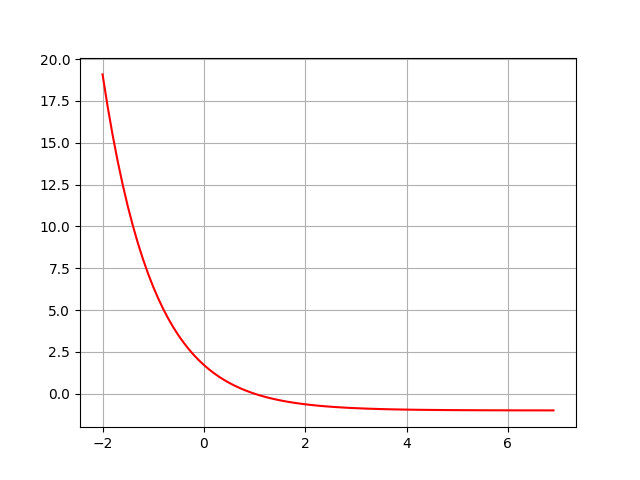
\includegraphics[totalheight=6cm]{../plots/ex6_f_1.png}
  \caption{Wykres $f_1(x) = e^{1 - x} - 1$}
\end{figure}

\begin{figure}[!htbp]
  \centering  
  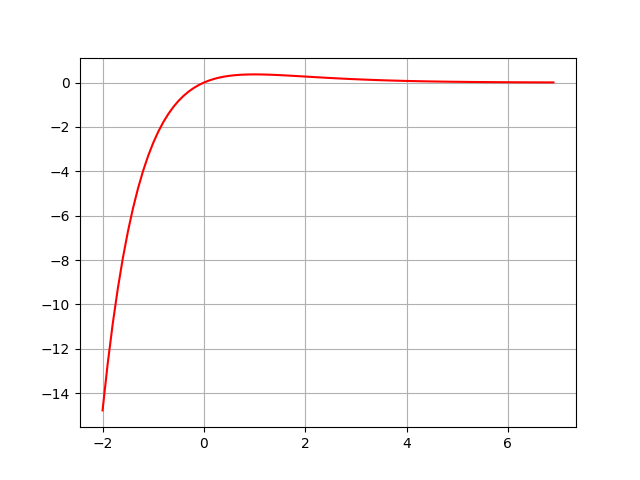
\includegraphics[totalheight=6cm]{../plots/ex6_f_2.png}
  \caption{Wykres $f_2(x) = xe^{-x}$}
\end{figure}


Z analizy wykresów (Rysunek 2, Rysunek 3) zaobserwowałem, że poszukiwane miejsca zerowe znajduje się w przypadku $ f_1(x) $ przedziale $ x \in [0.0, 2.0] $, a w przypadku $ f_2(x) $ przedziale $ x \in [-1.0, 1.0] $. Krańce tych przedziałów przyjąłem za punkty początkowe w przypadku obliczeń metodą siecznych, tych przedziałów użyłem również do wyliczenia wyniku metodą bisekcji. Za punkt początkowy, w przypadku metody stycznych, przyjąłem $ -0.5 $.
\newpage
\subsection{Wynik}
Wyniki zestawiłem w tabelach poniżej: \\
\begin{center}
Dla $f_1(x) = e^{1 - x} - 1$: \\
\end{center}

\begin{center}
  \begin{tabular}{|c|c|c|c|c|}
    \hline 
      Metoda & $x$ & $ f(x)$ & $i$ & $err$ \\
    \hline
    Bisekcja & 1.0 & 0.0 & 1 & 0\\
    \hline 
    Stycznych & 0.9999922654776594 & 7.734552252003368e-6 & 5 & 0\\
    \hline  
    Siecznych & 1.0000017597132702 & -1.7597117218937086e-6 & 6 & 0 \\
    \hline
  \end{tabular} 
\end{center}

\begin{center} 
Dla $f_2(x) = xe^{-x}$: \\
\end{center}

\begin{center}
  \begin{tabular}{|c|c|c|c|c|}
    \hline 
      Metoda & $x$ & $ f(x)$ & $i$ & $err$ \\
    \hline
    Bisekcja & 0.0 & 0.0 & 1 & 0\\
    \hline 
    Stycznych & -3.0642493416461764e-7 & -3.0642502806087233e-7 & 4 & 0\\
    \hline  
    Siecznych & 1.744165849924562e-8 & 1.7441658195034172e-8 & 18 & 0 \\
    \hline
  \end{tabular} 
\end{center}

\ \\
Podczas wyliczania miejsc zerowych funkcji przedstawionych w treści zadania zauważyłem, że wybór punktów w metodzie bisekcji zawsze doprowadzi nas do rozwiązania. Oczywiście wybranie punktów startowych odległych od miejsca zerowego o $ x_{00} = x_0 - \delta $ oraz $ x_{01} = x_0 + \delta $ w łatwy sposób pozwoli trafić w miejse zerowe. Przykładowe wyniki dla bisekcji dla lekko przesuniętych miejsc zerowych to odpowiednio \\dla $f_1 \rightarrow$ $ \mathtt{(0.999993896484375, 6.1035342515669555e-6, 16, 0)} $ \\dla $ f_2 \rightarrow $ $ \mathtt{(-3.051757812455591e-6, -3.051767125695548e-6, 17, 0)}$ \\ W kwestii zbieżności - globalna zbieżność odróżnia metodę bisekcji od reszty. W przypadku pozostałych dwóch - metody stycznych oraz metody siecznych, dobór punktów startowych jest istotnym elementem. Metody te są jedynie lokalnie zbieżne, a więc złe punkty początkowe nie doprowadzą do dobrego wyniku. Przykładem źle dobranych punktów startowych są zestawy parametrów startowych przedstawione w kolejnej sekcji.

\subsection{Dobór parametrów}

Dodatkowym punktem zadania było sprawdzenie zachowania metody Newtona dla pewnych parametrów:

\begin{enumerate}
  \item dla $ f_1 $ gdy $ x_0 > 1 $
  \item dla $ f_2 $ gdy $ x_0 > 0 $
  \item dla $ f_2 $ gdy $ x_0 = 1$
  
\end{enumerate}
\ \\
Analiza wywołań:

\begin{enumerate}
  \item W tym wypadku wartości zwracane przez metodę były akceptowalne do $ x_0 = 7.4 $. W kolejnych iteracjach testu $x_0 \in [7.6, 12.4] $ pojawił się błąd $ err = 1 $ (nieosiągnięto dokładności po $\mathtt{maxit}$ iteracjach), a wartości zwracane przez metodę to $ \mathtt{NaN} $. Powodem pojawienia się $ \mathtt{NaN} $ tj. (not a number) był fakt, że w pewnym momencie pochodna, bliska zeru, przechodziła przez test $|f'(x0)| < \epsilon $, ale w momencie, gdy algorytm wyliczał $ x_1 = x_0 - \frac{v}{f'(x0)} $, to dochodziło do dzielenia przez zero. Dalsze iteracje zwracały błąd $ err = 2$ świadczący o pochodnej bliskiej zeru - wtedy warunek $|f'(x0)| < \epsilon $ zwracał  $\mathtt{true}$ i metoda kończyła działanie.

  \item Sprawdzając kolejne wywołania metody Netwona dla parametrów $ x \in (0, \infty) $ zauważyłem, że do osiągnięcia $ x = 1.0 $, oscylowały w granicach realnej wartości. Przy $ x  = 1.0 $ funkcja zwróciła $ \mathtt{err = 2} $, kolejne obliczenia, dla $ x_0 > 1.0 $ zwracały wartości znacznie odbiegające od realnej.

  \item Po wywołaniu metody Newtona na $ f_2 $ z zadanymi paramterami otrzymujemy $ \mathtt{(1.0, -0.0, 0, 2)} $. Takie zachowanie (będące odstępstwem od punktów w otoczeniu tego punktu) związane jest z pochodną tej funkcji, tj. $ f_{2}'(x) = -e^{-x}(x - 1)$, która w $ x_0 = 1 $ osiąga swoje miejsce zerowe, a więc styczna $g(x) || OX$, tj. nie spełnia warunków metody Netwona.

\end{enumerate}
\ \\
Powyższe zestawy pokazują, że metody Netwona i siecznych są jedynie zbieżne lokalnie, a źle dobrane parametry początkowe uniemożliwiają osiągnięcie rozsądnych wyników. 

% Sprawdzić co stanie, gdy w metodzie Newtona dla f1 wybierzemy x0 ∈ (1, ∞] a dla f2 wybierzemy
% x0 > 1, czy mogę wybrać x0 = 1 dla f2?